\documentclass[sigconf,nonacm]{acmart}

\usepackage{booktabs}
\usepackage{multirow}
\usepackage{pgfplots}
\pgfplotsset{compat=1.17}
\usepackage{algorithm}
\usepackage{algpseudocode}

\settopmatter{printacmref=false}
\setcopyright{none}
\renewcommand\footnotetextcopyrightpermission[1]{}

\setlength{\emergencystretch}{2em}
\newcommand{\Z}{\mathbb{Z}}
\newcommand{\R}{\mathcal{R}}
\newcommand{\lgqp}{\log_2(q_0 p')}

\begin{document}

\title{Shallow CKKS Bootstrapping in Practice}
\subtitle{An Open-Source OpenFHE Implementation of SHIP, a Security Re-evaluation of its Sparse-Key Parameters, and a Same-Machine Comparison}

\author{WooYoung Choi}
\affiliation{%
  \institution{Korea University}
  \city{Seoul}
  \country{Republic of Korea}}

\begin{abstract}
SHIP (Cheon, Hanrot, Kim and Stehl\'e, EUROCRYPT 2025) is a CKKS bootstrapping algorithm that replaces the top-level homomorphic DFT and the polynomial approximation of modular reduction by $h$ independent blind rotations and a product tree.
Its bootstrapping depth is only $6$ levels for a sparse secret of Hamming weight $h=31$, which makes full-slot bootstrapping possible in ring degree $N=2^{13}$ at 128-bit security.
The original evaluation used an experimental implementation on top of the HEaaN library.
We report, to the best of our knowledge, the first publicly available implementation of SHIP, integrated into OpenFHE as a library feature with a \texttt{CryptoContext} API, key serialization, seed-compressed keys and disk-backed keys.
Reproducing the four parameter sets of the paper, we obtain single-thread latencies within $8\%$ of the published single-core figures and precisions within $0.9$ bits for three of the four sets.
Two observations go beyond reproduction.
First, at the small scaling factors that SHIP enables ($2^{20}$--$2^{24}$), the approximate RNS ModDown of hybrid key switching introduces a biased rounding error that destroys the output; we replace it by an exact centered rounding behind OpenFHE's existing \texttt{WITH\_REDUCED\_NOISE} flag.
Second, running the current lattice estimator on the sparse-key switching key, two of the three published 128-bit bounds evaluate to $2^{121.4}$ and $2^{126.2}$ under the primal hybrid meet-in-the-middle attack; lowering $\lgqp$ from $55$ to $42$ and from $100$ to $88$ restores at least $2^{129.8}$ without measurable precision loss for LL14.
Finally, we compare SHIP with OpenFHE's bootstrapping tuned with the same sparse-secret encapsulation on the same machine.
SHIP's latency is $2.0\times$ (one thread) to $4.2\times$ (15 threads) lower and its memory footprint is about half, while the tuned baseline at $N=2^{16}$ has $2$ more bits of precision and $1.1$--$2.3\times$ higher throughput.
SHIP is therefore the right tool when latency, ring degree or memory is the constraint, not when throughput is.
\end{abstract}

\keywords{Fully homomorphic encryption, CKKS, bootstrapping, OpenFHE, sparse-secret LWE, lattice estimator}

\maketitle

%=====================================================================
\section{Introduction}
%=====================================================================

CKKS~\cite{CKKS17} offers high-throughput approximate arithmetic on encrypted vectors, but its bootstrapping~\cite{CHKKS18} is expensive in latency.
The conventional procedure evaluates a homomorphic DFT at the top modulus, a polynomial approximation of the modular reduction, and an inverse DFT.
These steps consume $12$ to $21$ multiplicative levels, which forces a large modulus and therefore ring degree $N\ge 2^{16}$ at 128-bit security when full-slot bootstrapping with good precision is needed.

SHIP~\cite{CHKS25} changes this balance.
Writing the decryption equation $a s + b = m \bmod q_0$ coefficient-wise, it computes $\omega^{m_i}$ with $\omega=e^{2\pi\iota/q_0}$ as a product of $h$ factors, one per nonzero coefficient of a sparse secret of Hamming weight $h$.
Each factor is obtained by a \emph{blind rotation} of public phases by an encrypted index, and the $h+1$ factors are multiplied in a binary tree.
Only the tree consumes levels, $\lceil\log_2(h+1)\rceil=5$ for $h=31$, plus one level for the slots-to-coefficients transform (S2C).
With $6$ levels, the authors report the first CKKS-only full-slot bootstrapping at $N=2^{13}$, $215$\,ms on $32$ cores, and good multi-core scaling, because the $h$ factors are independent.

The original evaluation used an experimental implementation on the HEaaN library~\cite{HEaaN}.
To our knowledge no public implementation exists, and several practical questions are open: how SHIP behaves inside a general-purpose library whose key-switching and scaling conventions were designed for $40$--$60$-bit primes; whether its sparse-key parameters remain secure under current attack estimates; how large and how portable its keys are; and how it compares with a \emph{tuned} conventional bootstrapping on the same machine.

\paragraph{Contributions}
\begin{itemize}
\item \textbf{Implementation (\S\ref{sec:impl}).} We implement SHIP in OpenFHE~\cite{OpenFHE22} as a library feature: column-plus-mux blind rotations with base-$4$ multiplexers and hoisting, the windowed sparse secret, masks multiplied at the auxiliary modulus (no masking level), sparse-secret encapsulation at modulus $q_0p'$, a one-level dense S2C, and role-specific primes as in the paper's Table~2. The library adds key serialization, seed-compressed keys ($0.50\times$ size) and disk-backed keys that make the $70$\,GiB HT15 key usable on a $48$\,GB machine.
\item \textbf{A rounding bias at small scales (\S\ref{sec:moddown}).} OpenFHE's approximate ModDown floors instead of rounding and adds a $\pm1$ error per coefficient for multi-prime $P$. Multiplied by a dense secret, this becomes a biased error of tens of units per coefficient, which at SHIP's $2^{20}$ scale reduces LL13 to an error of $1.5$--$5$. We implement exact centered rounding behind \texttt{WITH\_REDUCED\_NOISE}; all $2{,}119$ OpenFHE unit tests pass.
\item \textbf{Security re-evaluation (\S\ref{sec:security}).} With the current lattice estimator~\cite{APS15,estimator}, the sparse-key bounds $(\log N,\lgqp)=(13,55)$ and $(14,100)$ give $2^{121.4}$ and $2^{126.2}$ under the primal hybrid meet-in-the-middle attack. We lower the defaults to $42$ and $88$ ($2^{129.8}$ and $2^{130.2}$); $(15,105)$ stays at $2^{148.7}$.
\item \textbf{Same-machine evaluation (\S\ref{sec:eval}).} We reproduce LL13, LL14, HT14 and HT15, and compare against OpenFHE's \texttt{EvalBootstrap} tuned with the same sparse-secret encapsulation~\cite{BTH22}, at $1$, $4$ and $15$ threads. We also quantify the cost of noise flooding for IND-CPA$^D$ security~\cite{LM21}.
\end{itemize}
The code, unit tests, raw logs and estimator scripts are public~\cite{ShipCode}.

%=====================================================================
\section{Background}
\label{sec:background}
%=====================================================================

\paragraph{CKKS and RNS}
We use the RNS variant of CKKS with ciphertext modulus $Q=\prod_{i=0}^{L} q_i$, auxiliary modulus $P$ for hybrid key switching with $d_{\mathrm{num}}$ digits, ring $\R=\Z[X]/(X^N+1)$ and $N/2$ complex slots.
With OpenFHE's \texttt{FIXEDMANUAL} scaling, every rescaling prime is assumed equal to the scaling factor $\Delta=2^p$.
Security of the dense (uniform ternary) secret follows the HE standard~\cite{HEStd18}, which bounds $\log_2(QP)$ for each $N$ (e.g.\ $218$, $438$, $881$ bits for $N=2^{13},2^{14},2^{15}$).

\paragraph{Sparse-secret encapsulation}
Bootstrapping algorithms prefer a sparse secret at the bottom modulus, but sparse secrets weaken the RLWE instance.
Bossuat et al.~\cite{BTH22} keep the dense secret for the whole computation and switch to a sparse secret only for the ModRaise step, with a switching key at a small modulus $q_0 p'$.
Only that one key involves the sparse secret, so only $\lgqp$ needs to satisfy the sparse-secret security bound.
OpenFHE exposes this technique as \texttt{SPARSE\_ENCAPSULATED} ($h=32$, key modulus $q_0p_0$), and SHIP uses it with $h=31$.

\paragraph{SHIP}
Let $(a,b)\in\R_{q_0}^2$ decrypt to $m$ under a sparse secret $s$ with nonzero coefficients $s_{j_1},\dots,s_{j_h}\in\{\pm1\}$, and let $\gamma=q_0/\Delta$.
For every coefficient $i$,
\[
\omega^{m_i} = \omega^{b_i}\prod_{k=1}^{h}\omega^{\pm a_{i-j_k} s_{j_k}},
\]
with signs from the negacyclic reduction.
SHIP evaluates this product for all $N/2$ slots at once~\cite[Alg.~1]{CHKS25}:
(i)~the public phases $\omega^{\pm a}$ are encoded in four half-vectors;
(ii)~for each nonzero $s_{j_k}$, encrypted masks that depend on $(j_k,s_{j_k})$ select and sign the right halves (Lemma~1 of~\cite{CHKS25});
(iii)~a blind rotation by the encrypted index $j_k$ aligns the factor;
(iv)~a product tree multiplies the $h$ factors and the public $\omega^{b}$ term;
(v)~adding the complex conjugate yields $\frac{\gamma}{2\pi}\sin(2\pi m_i/\gamma)\approx m_i\Delta$ in the slots.
The blind rotation combines a \emph{column} method, where the masks are pre-rotated for the $\theta$ candidate offsets of a window, and a \emph{mux} method, where encrypted digits in base $B$ drive $B$-to-$1$ multiplexed rotations (HMuxRot)~\cite[Def.~1, Alg.~3--5]{CHKS25}.
To bound the rotation range, the secret is sampled with one nonzero coefficient per window: the $k$-th lies in $[kN/h-w,\,kN/h+w)$, so only $2w$ positions must be covered.
The security of this structure is argued with May's meet-LWE estimate~\cite{May21}, $(4w)^{0.4h}\ge 2^{115}$~\cite[\S5.1]{CHKS25}.
Masks are multiplied at modulus $QP$ with scale $P$ and removed by the ModDown of key switching, so masking consumes no level~\cite[\S4.1, \S4.4]{CHKS25}.
Before the blind rotations, a dense S2C at the bottom modulus moves the slots into coefficients with one level~\cite[\S3.2]{CHKS25}.

The paper defines four parameter sets~\cite[Table~2]{CHKS25}: LL13 and LL14 (low latency, one multiplicative level after bootstrapping) and HT14 and HT15 (high throughput, nine levels).

%=====================================================================
\section{Implementation in OpenFHE}
\label{sec:impl}
%=====================================================================

The implementation is a new module \texttt{ckksrns-ship} (about $1{,}400$ lines of C++) in OpenFHE~1.4.2, plus five methods on \texttt{CryptoContext}:
\begin{verbatim}
auto spec = SHIPContextSpec::LL14();
auto cc   = GenSHIPCryptoContext(spec);
auto kp   = cc->KeyGen();
cc->EvalMultKeyGen(kp.secretKey);
auto prm  = SHIPParams::Recommended(spec);
cc->EvalSHIPBootstrapKeyGen(kp.secretKey, prm);
auto out  = cc->EvalSHIPBootstrap(ct);
\end{verbatim}
\texttt{GenSHIPCryptoContext} builds the modulus chain and throws if $\log_2(QP)$ exceeds the HE-standard bound.
The bootstrapping input is a fully packed, rescaled ciphertext with at least two limbs; the output has the full chain minus the five product-tree levels.

\subsection{Data flow}
\texttt{EvalSHIPBootstrap} (Algorithm~\ref{alg:ship}) (1)~drops the input to two limbs, (2)~applies the dense S2C with a baby-step giant-step diagonal method, consuming one level, (3)~switches to the sparse secret at modulus $q_0p'$, and (4)~runs the half bootstrap of Algorithm~1 for real messages (twice for complex messages).
In the half bootstrap, the $h=31$ factors are computed in an OpenMP parallel loop.
For each factor, the four public phase polynomials are lifted from $q_0$ to all limbs of $QP$, rotated to the $\theta$ column offsets, multiplied by the column keys $\mathrm{Enc}_{QP}(P\cdot\text{mask})$, summed, and reduced by one ModDown.
The result enters the mux part: $\lceil\log_B\lceil 2w/\theta\rceil\rceil$ steps (three in all presets), each a $B$-to-$1$ mux-rotate whose $B$ branches share one gadget decomposition and one ModDown.
The product tree then multiplies the $32$ terms, and the public term $\omega^b$ enters as a trivial ciphertext, so evaluation needs no public key.

\begin{algorithm}[t]
\caption{\texttt{EvalSHIPBootstrap} for real messages}
\label{alg:ship}
\small
\begin{algorithmic}[1]
\Require fully packed ciphertext $ct$ with $\ge 2$ limbs; SHIP key with factor keys $C_k$, $M_k$ ($1\le k\le h$)
\State $ct \gets$ \textsc{LevelReduce}$(ct)$ to two limbs
\State $ct \gets$ \textsc{S2C}$(ct)$ \Comment{one level; now modulo $q_0$}
\State $(a,b) \gets$ \textsc{Encapsulate}$(ct)$ \Comment{dense $\to$ sparse at $q_0p'$}
\State $\phi_{1..4} \gets$ halves of $\omega^{\pm a}$, encoded at $q_0$ and lifted to $QP$
\State $T_0 \gets$ trivial ciphertext of $\frac{\gamma K}{4\pi\iota\kappa}\,\omega^{b}$ \Comment{$K$: input bound}
\ForAll{$k=1,\dots,h$ \textbf{in parallel}}
  \State $c \gets \sum_{t<\theta}\sum_{u=1}^{4} \textsc{Rot}_{o_k+t}(\phi_u)\cdot C_{k,t,u}$ \Comment{at $QP$}
  \State $c \gets \textsc{ModDown}_P(c)$ \Comment{masking uses no level}
  \For{each of the $\lceil\log_B\lceil 2w/\theta\rceil\rceil$ mux steps $\ell$}
    \State $c \gets \textsc{MuxRot}_B(c, M_{k,\ell})$ \Comment{shared decomposition}
  \EndFor
  \State $T_k \gets c$
\EndFor
\State $R \gets \textsc{ProductTree}(T_0,\dots,T_h)$ \Comment{$\lceil\log_2(h+1)\rceil$ levels}
\State \Return $R + \textsc{Conj}(R)$
\end{algorithmic}
\end{algorithm}

\subsection{Role-specific primes and exact output scale}
\label{sec:primes}
Table~2 of~\cite{CHKS25} assigns different prime sizes to the base prime, the S2C prime, the user's multiplicative primes, the bootstrapping (product-tree) primes and the auxiliary primes.
We build the chain with \texttt{ILDCRTParams} and choose for each role the NTT-friendly prime closest to the target size.
Two corrections make this work under \texttt{FIXEDMANUAL}:
\begin{itemize}
\item The product tree is computed at scale $2^{b}$ with $b>p$, while downstream code expects $2^{p}$. We set the last tree prime to $2b-p$ bits so that the root returns to scale $2^p$.
\item Small NTT-friendly primes deviate from $2^b$ by a few percent, and the deviation compounds through five tree levels. Because all leaves enter at the same level with known scale, the true root scale $\kappa\cdot 2^p$ is deterministic; we simulate the pairing of the tree once and fold $1/\kappa$ into the public plaintext $\omega^b$. Likewise, the S2C diagonals are multiplied by $q/\Delta$ for the exact prime $q$ they are rescaled by.
\end{itemize}
OpenFHE fixes the size of $P$ primes at $60$ bits; to fit LL13's $218$-bit budget, the SHIP context regenerates the CRT tables with the requested auxiliary prime size.

\subsection{Keys}
\label{sec:keys}
A SHIP key consists of, per nonzero coefficient, $4\theta$ column ciphertexts at $QP$ and the mux keys of each step; plus S2C rotation keys, the conjugation key and the encapsulation key.
Its size is dominated by the factor keys: $h\,(4\theta + 3B\,d_{\mathrm{num}})$ polynomial pairs at modulus $QP$.
Table~\ref{tab:keys} lists the predicted sizes.
We implemented three measures:
\begin{itemize}
\item \textbf{SHIP-owned switching keys with level truncation.} S2C and conjugation keys are only used at one known level, so their digits and limbs are restricted to that level.
\item \textbf{Seed compression.} Every uniform component $a$ of a switching key is derived from a per-key random seed (BLAKE2) and an identifier. The compact serialization stores only the $b$ components and regenerates $a$ on loading; the serialized size is $0.500\times$ the full size in our tests. This is the standard trade-off of seeded public keys: the seed is public information, and both sides must use the same PRNG.
\item \textbf{Disk-backed factor keys.} With a directory argument, the factor keys are written to one file per factor during key generation and streamed during bootstrapping, so only the S2C, conjugation and encapsulation keys stay in memory. This is how HT14 and HT15 run on our $48$\,GB machine.
\end{itemize}

\begin{table}[t]
\caption{Parameter sets as implemented (all within the HE-standard $\log_2(QP)$ bound). Bits are prime sizes; ``boot'' are the product-tree primes. Key sizes are predicted by \texttt{SHIPEstimateKeyBytes}.}
\label{tab:keys}
\small
\begin{tabular}{lrrrr}
\toprule
 & LL13 & LL14 & HT14 & HT15 \\
\midrule
$N$ & $2^{13}$ & $2^{14}$ & $2^{14}$ & $2^{15}$ \\
$\log_2(QP)$ / bound & 218/218 & 437/438 & 434/438 & 827/881 \\
$d_{\mathrm{num}}$ & 8 & 4 & 8 & 6 \\
base, S2C & 25, 20 & 48, 37 & 28, 23 & 51, 39 \\
user levels (bits) & 1 (21) & 1 (37) & 9 (23--24) & 9 (39--40) \\
boot primes & 24--28 & 42--48 & 24--25 & 46--54 \\
$P$ & 28 & 50, 50 & 55 & $3\times 50$ \\
$w$, $\theta$, $B$ & 175, 6, 4 & 264, 9, 4 & 264, 9, 4 & 528, 17, 4 \\
$\lgqp$ (default) & 42 & 88 & 88 & 105 \\
key (GiB) & 8.0 & 12.2 & 31.5 & 69.6 \\
\bottomrule
\end{tabular}
\end{table}

\subsection{Input range}
SHIP computes $\frac{\gamma}{2\pi}\sin(2\pi m/\gamma)$, which is close to $m$ only for $|m|\lesssim 1$ in message units.
A parameter \texttt{messageBound}~$K$ divides the message by $K$ inside the S2C diagonals and multiplies it back through the public plaintext $\omega^b$, at no level cost and about $\log_2 K$ bits of precision.
On inputs in $[-64,64]$, $K=1$ gives a maximum error of $1.62$ (the sine approximation fails) and $K=64$ gives $4.0\times10^{-4}$.

\subsection{Testing}
Nine unit tests cover real and complex messages, windowed and unrestricted secrets, base-$2$ and base-$4$ mux, role-specific primes, inputs at higher levels, invalid inputs and keys, compact serialization round trips, disk-backed keys, the input range, and the HE-standard check of the four presets.
A client--server example generates and serializes the key on one side and bootstraps, squares and bootstraps again on the other.

%=====================================================================
\section{Exact Rounding in ModDown}
\label{sec:moddown}
%=====================================================================

Hybrid key switching ends with $\mathrm{ModDown}$: given $x$ over $QP$, compute $\lfloor x/P\rceil$ over $Q$.
OpenFHE's \texttt{ApproxModDown} computes $[x]_P$ by an approximate fast basis conversion to the $Q$ primes, $\tilde r=\sum_j [y_j \hat P_j^{-1}]_{p_j}\hat P_j$ with $\hat P_j=P/p_j$, and returns $(x-\tilde r)/P$.
Two effects make this a biased estimate of $x/P$:
\begin{enumerate}
\item $[x]_P\in[0,P)$, so the division is a floor, not a rounding; the error has mean $1/2$.
\item $\tilde r = [x]_P + \alpha P$ with $\alpha\in[0,k)$ for $k$ auxiliary primes, which adds an error of up to $k-1$ per coefficient.
\end{enumerate}
In key switching these errors are multiplied by the secret.
With a dense ternary secret, a constant error of $1/2$ per coefficient becomes a low-frequency error whose coefficients are sums of hundreds of terms, concentrated in slot~$0$.
At scale $2^{40}$ or more it is invisible.
SHIP, however, works at $2^{20}$--$2^{24}$ in LL13 and performs hundreds of key switches per bootstrapping.
In our diagnostics, every factor carried a slot-$0$ error of $0.02$--$0.25$, and the final error was $0.8$--$5$.

When OpenFHE is built with \texttt{WITH\_REDUCED\_NOISE} and the plaintext modulus is $t=0$ (CKKS, BFV), we compute the centered remainder exactly:
\[
r=\sum_j y_j \hat P_j - \Big\lfloor \sum_j \tfrac{y_j}{p_j} \Big\rceil P,\qquad y_j=[x\,\hat P_j^{-1}]_{p_j},
\]
with a $128$-bit accumulator and Barrett reduction, so that $(x-r)/P=\lfloor x/P\rceil$.
BGV ($t>0$) and builds without the flag are unchanged.

\begin{table}[t]
\caption{Effect of exact rounding in ModDown on SHIP precision (bits; ``error'' is the maximum slot error when precision is below 0).}
\label{tab:moddown}
\small
\begin{tabular}{p{3.6cm}p{1.6cm}p{1.9cm}}
\toprule
Setting & default & exact rounding \\
\midrule
LL13, uniform 22-bit primes, 28-bit $P$ & error 1.5--5 & 1.3--1.6 bits \\
LL13, same primes, 60-bit $P$ & error 0.55--2.5 & 3.3 bits \\
LL14, uniform 40-bit primes & 13.8--13.9 bits$^{*}$ & 14.4 bits \\
Role-specific primes (\S\ref{sec:primes}) & -- & LL13 2.3--2.5, LL14 16.1--16.5 \\
\bottomrule
\end{tabular}

\smallskip
\footnotesize $^{*}$With \texttt{WITH\_REDUCED\_NOISE} before the rounding change.
\end{table}

Table~\ref{tab:moddown} shows the effect.
With the change, the full OpenFHE suites (core $156$, binfhe $78$, pke $1{,}885$ tests, including the SHIP tests) pass with the flag enabled.
The fix is relevant beyond SHIP for any CKKS use of small scales.

%=====================================================================
\section{Security Re-evaluation}
\label{sec:security}
%=====================================================================

SHIP involves three secrets: the dense ternary secret of all evaluation keys at modulus $QP$, the sparse secret of the single encapsulation key at modulus $q_0p'$, and the windowed position structure of that sparse secret.
We ran the lattice estimator~\cite{estimator} (commit \texttt{d8c00b48}, 2026-08-19, SageMath~10.5) with error $\sigma=3.19$; the sparse secret is modelled as $16$ coefficients $+1$ and $15$ coefficients $-1$.

\paragraph{Dense keys}
Table~\ref{tab:dense} compares the dense keys with the HE-standard boundary at the same $N$.
The current estimator rates the standard boundary itself at about $2^{126}$, and our contexts are at or above it; ``128-bit'' for dense keys therefore means ``within the HE-standard table'', as in the paper.

\begin{table}[t]
\caption{Dense keys: $\log_2$ of the attack cost.}
\label{tab:dense}
\small
\begin{tabular}{lrrrr}
\toprule
Set & $\log_2(QP)$ & uSVP & dual hybrid & HE-std boundary \\
\midrule
LL13 & 218 & 126.0 & 126.5 & 218 $\to$ 126.0 \\
LL14 & 437 & 126.2 & 126.9 & 438 $\to$ 125.9 \\
HT14 & 434 & 127.3 & 128.1 & 438 $\to$ 125.9 \\
HT15 & 827 & 134.7 & 135.7 & 881 $\to$ 126.1 \\
\bottomrule
\end{tabular}
\end{table}

\paragraph{Sparse key}
The paper states that the pairs $(\log N,\log(Pq_0))=(13,55)$, $(14,100)$ and $(15,105)$ give 128-bit security for $h=31$~\cite[\S5.2]{CHKS25}.
For these small moduli, uSVP and the dual hybrid attack either do not apply or cost more than $2^{300}$; the best attack is the primal hybrid with meet-in-the-middle guessing that \texttt{LWE.estimate} reports as \texttt{bdd\_mitm\_hybrid}.
Table~\ref{tab:sparse} shows the results.
Two of the three published points fall below $2^{128}$.
Restricting the number of samples to $m=n$ (one RLWE sample) gives the same $2^{121.4}$ for $(13,55)$.
We cannot tell which estimator version and attack set the original analysis used; hybrid attacks on sparse secrets have been revised several times~\cite{SC19,CP19,SecGuide24,PV25}, and the difference is consistent with that history.

\begin{table}[t]
\caption{Sparse encapsulation key ($h=31$): $\log_2$ cost of the primal hybrid MITM attack. Bold: library defaults.}
\label{tab:sparse}
\small
\begin{tabular}{rrrl}
\toprule
$N$ & $\lgqp$ & cost & note \\
\midrule
$2^{13}$ & 55 & 121.4 & paper bound \\
$2^{13}$ & 45 & 127.6 & \\
$2^{13}$ & \textbf{42} & \textbf{129.8} & default \\
$2^{14}$ & 100 & 126.2 & paper bound \\
$2^{14}$ & 92 & 128.9 & \\
$2^{14}$ & \textbf{88} & \textbf{130.2} & default (LL14, HT14) \\
$2^{15}$ & \textbf{105} & \textbf{148.7} & paper bound, default \\
\midrule
$2^{15}$ & 112 & 149.7 & OpenFHE baseline, $h=32$ \\
$2^{16}$ & 120 & 172.1 & OpenFHE baseline, $h=32$ \\
\bottomrule
\end{tabular}
\end{table}

\paragraph{New defaults}
We set the bound to $42$, $88$ and $105$ bits for $N=2^{13},2^{14},2^{15}$; \texttt{SHIPParams::Recommended} chooses the size of $p'$ from the actual $q_0$, and the minimum size of $p'$ is lowered to $17$ bits so that LL13 ($25$-bit $q_0$) fits.
For LL14, precision is unchanged ($16.0$--$16.5$ bits over $15$ runs with $p'=40$ bits).
For LL13, the worst of $15$ runs was $1.9$ bits, against $2.2$ bits with the previous $p'$; the smaller $p'$ adds key-switching noise in the encapsulation.
HT14 already used $88$ and HT15 is unchanged.

\paragraph{Windowed positions}
The estimator does not model one-nonzero-per-window secrets.
We keep the paper's criterion $(4w)^{0.4h}\ge 2^{115}$~\cite{May21,CHKS25}, which gives $2^{117.2}$ for LL13, $2^{124.6}$ for LL14 and HT14, and $2^{137.0}$ for HT15.
We have not analyzed this structure further and flag it as the least conservative part of the parameter sets.

%=====================================================================
\section{Evaluation}
\label{sec:eval}
%=====================================================================

\paragraph{Setup}
Apple M5 Pro ($15$ cores, mixed performance and efficiency cores), $48$\,GB RAM, macOS (arm64), AppleClang, OpenFHE~1.4.2 with \texttt{NATIVE\_SIZE=64}, \texttt{WITH\_REDUCED\_NOISE=ON} and OpenMP (Homebrew libomp).
Inputs are uniform real vectors in $[-1,1]$; precision is $\log_2(1/\varepsilon)$ with $\varepsilon$ the maximum real error over all slots, as in~\cite{CHKS25}.
Latency excludes key generation.
OpenFHE caches its thread count at start-up, so every thread count runs in a separate process with \texttt{OMP\_NUM\_THREADS} set.
Unless stated otherwise, measurements were taken with no other heavy workload; we report medians of $5$ runs (SHIP) or $3$ runs (baseline).
Throughput follows~\cite[Eq.~(9)]{CHKS25}: slots $\times$ levels after bootstrapping $\times$ precision / latency, using the worst precision.

\subsection{Reproduction}
Table~\ref{tab:repro} compares our LL13 and LL14 results with the paper.
Single-thread latency is within $8\%$ of the published single-core numbers, and four threads are within $13\%$ of the published four-core numbers, on a different CPU and library.
LL14 precision is $0.4$--$0.9$ bits below the paper.
LL13 precision is $2.0$--$2.6$ bits below.
We traced the LL13 gap to the dense-key encryption noise: with OpenFHE's uniform ternary key at $N=2^{13}$ and scale $2^{20}$, plain encryption followed by decryption already has a maximum slot error of $0.10$--$0.11$ (mean $0.024$), larger than the paper's total LL13 error ($2^{-4.45}\approx0.046$).
We did not compare with HEaaN's key distribution directly.

\begin{table}[t]
\caption{Reproduction of the low-latency sets. Ours: median [min--max] of 5 runs. Paper: HEaaN on AMD EPYC 7473X.}
\label{tab:repro}
\small
\begin{tabular}{lll}
\toprule
 & LL13 & LL14 \\
\midrule
precision (ours) & 1.9--2.5 & 16.0--16.5 \\
precision (paper) & 4.45 & 16.9 \\
1 thread (ours) & 2.98\,s [2.97--3.14] & 5.28\,s [5.24--5.74] \\
1 core (paper) & 3.02\,s & 4.91\,s \\
4 threads (ours) & 0.90\,s [0.87--0.92] & 1.45\,s [1.41--1.48] \\
4 cores (paper) & 0.80\,s & 1.29\,s \\
15 threads (ours) & 0.58\,s ($5.1\times$) & 0.83\,s ($6.4\times$) \\
32 cores (paper) & 215\,ms & 333\,ms \\
key generation & 17\,s & 24--26\,s \\
max RSS & 8.6\,GiB & 13.8\,GiB \\
\bottomrule
\end{tabular}
\end{table}

\paragraph{High-throughput sets}
HT14 and HT15 were run with disk-backed factor keys (internal SSD) at four threads, two runs each, while another application was running; their latencies include reading tens of gigabytes of keys and are not comparable with the paper.
HT15 reaches $18.3$--$18.4$ bits (paper: $18.1$) with nine multiplicative levels left, in $49$--$51$\,s; key generation takes $354$\,s, $8.6$\,GiB of the $69.6$\,GiB key stays in memory and the maximum RSS is $27.3$\,GiB.
HT14 reaches $4.0$ bits (paper: $4.55$) with nine levels, in $8$--$19$\,s, maximum RSS $14.4$\,GiB.
The precision and level counts confirm that the parameter sets are reproduced; their speed needs a machine with enough memory.

\subsection{Comparison with tuned OpenFHE bootstrapping}

A fair baseline must use the same security level, the same number of levels left (one) and the techniques that are standard today.
With OpenFHE's default uniform ternary secret, \texttt{EvalBootstrap} needs $19$--$21$ levels; at $N=2^{15}$ decryption fails because of the approximation error, and at $N=2^{16}$ we obtained $5.3$--$10.6$ bits in $11.5$--$30.3$\,s on one thread.
That baseline is too weak.
We therefore enabled \texttt{SPARSE\_ENCAPSULATED}~\cite{BTH22}, which is the same encapsulation idea that SHIP uses and whose sparse key is above $2^{149}$ (Table~\ref{tab:sparse}).
At $N=2^{15}$, OpenFHE requires $\log_2(q_0/\Delta)\le 7$ and the $881$-bit budget limits the scale to $45$ bits; with scale $40$ the precision was one bit.
At $N=2^{16}$ we used OpenFHE's recommended $59/60$-bit scale with level budget $(2,2)$.

\begin{table*}[t]
\caption{Same-machine comparison (128-bit, one multiplicative level after bootstrapping). Latency: median of 5 (SHIP) or 3 (OpenFHE) runs. Throughput: slots $\times$ levels $\times$ precision / latency, in thousands. Key generation includes OpenFHE's bootstrapping setup.}
\label{tab:compare}
\small
\begin{tabular}{lrrrrrrrrrrr}
\toprule
 & & & & \multicolumn{3}{c}{latency (s)} & \multicolumn{3}{c}{throughput ($10^3$)} & keygen & max \\
\cmidrule(lr){5-7}\cmidrule(lr){8-10}
Method & $N$ & slots & precision & 1 thr & 4 thr & 15 thr & 1 thr & 4 thr & 15 thr & 1 thr (s) & RSS (GiB) \\
\midrule
SHIP LL13 & $2^{13}$ & 4{,}096 & 1.9--2.5 & 2.98 & 0.90 & 0.58 & 3 & 10 & 13 & 17 & 8.6 \\
SHIP LL14 & $2^{14}$ & 8{,}192 & 16.0--16.5 & \textbf{5.28} & \textbf{1.45} & \textbf{0.83} & 25 & 90 & 158 & 26 & 13.8 \\
OpenFHE sparse-enc., 45/52 & $2^{15}$ & 16{,}384 & 6.7--7.2 & 4.89 & 2.44 & 1.85 & 23 & 47 & 61 & 50 & 17.3 \\
OpenFHE sparse-enc., 59/60 & $2^{16}$ & 32{,}768 & \textbf{18.3--18.7} & 10.48 & 5.00 & 3.48 & \textbf{58} & \textbf{121} & \textbf{173} & 52 & 25.3 \\
\bottomrule
\end{tabular}
\end{table*}

\begin{figure}[t]
\centering
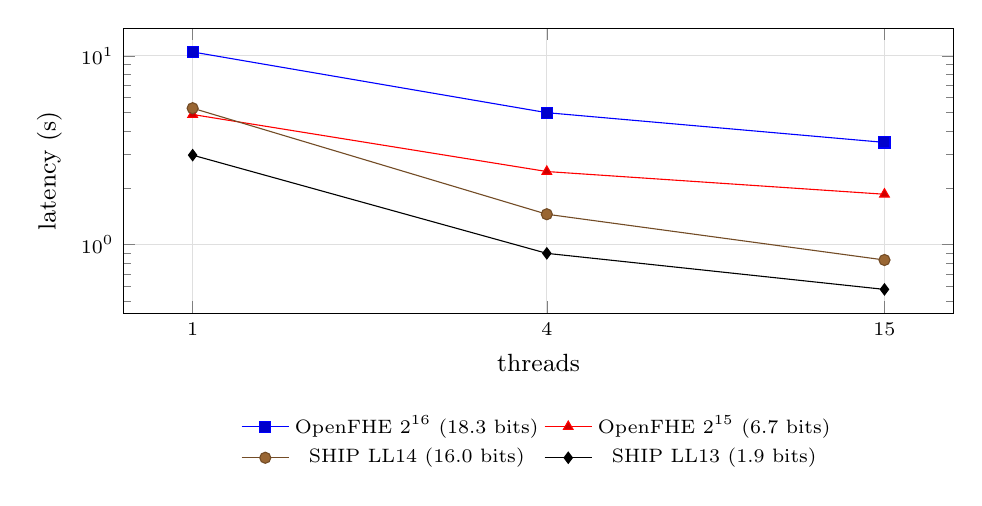
\begin{tikzpicture}
\begin{axis}[
  width=\columnwidth, height=5.2cm,
  xmode=log, ymode=log, log basis x=2,
  xtick={1,4,15}, xticklabels={1,4,15},
  xlabel={threads}, ylabel={latency (s)},
  legend style={font=\scriptsize, at={(0.5,-0.32)}, anchor=north, draw=none},
  legend columns=2,
  grid=major, grid style={gray!25},
  tick label style={font=\scriptsize}, label style={font=\small}]
\addplot+[mark=square*] coordinates {(1,10.48) (4,5.00) (15,3.48)};
\addlegendentry{OpenFHE $2^{16}$ (18.3 bits)}
\addplot+[mark=triangle*] coordinates {(1,4.89) (4,2.44) (15,1.85)};
\addlegendentry{OpenFHE $2^{15}$ (6.7 bits)}
\addplot+[mark=*] coordinates {(1,5.28) (4,1.45) (15,0.83)};
\addlegendentry{SHIP LL14 (16.0 bits)}
\addplot+[mark=diamond*] coordinates {(1,2.98) (4,0.90) (15,0.58)};
\addlegendentry{SHIP LL13 (1.9 bits)}
\end{axis}
\end{tikzpicture}
\Description{Log-log plot of bootstrapping latency against 1, 4 and 15 threads for SHIP LL13, SHIP LL14 and OpenFHE bootstrapping at N=2^15 and N=2^16. The SHIP curves are lower and steeper.}
\caption{Bootstrapping latency versus threads (log-log). SHIP scales better because its $h$ factors are independent.}
\label{fig:scaling}
\end{figure}

Table~\ref{tab:compare} and Figure~\ref{fig:scaling} show the results.
\begin{itemize}
\item \textbf{Latency.} LL14 is $2.0\times$, $3.4\times$ and $4.2\times$ faster than the $N=2^{16}$ baseline at $1$, $4$ and $15$ threads. The gap grows with the thread count because SHIP's $31$ factors are independent, while the baseline's linear transforms and polynomial evaluation have less coarse-grained parallelism. From $1$ to $15$ threads, LL14 speeds up $6.4\times$ and the baseline $3.0\times$.
\item \textbf{Precision.} The $N=2^{16}$ baseline has about two more bits. At $N=2^{15}$ the baseline reaches only $7$ bits, whereas SHIP's HT15 reaches $18.3$ bits at the same $N$.
\item \textbf{Throughput.} The $N=2^{16}$ baseline is $2.3\times$, $1.3\times$ and $1.1\times$ higher, because it refreshes four times as many slots. Only at $15$ threads does SHIP come close.
\item \textbf{Memory.} LL14 needs about half the memory ($13.8$ vs.\ $25.3$\,GiB), but its key must be transferred: $12.2$\,GiB, or about $6$\,GiB with seed compression.
\end{itemize}
We fixed one level after bootstrapping for both methods; the baseline can keep more levels at a modest cost, which raises its throughput further (the HEaaN baseline in~\cite[Table~3]{CHKS25} keeps nine).
Measurements taken earlier on the same machine under a concurrent gaming workload gave the same ordering for latency but large variance, and are not used.

\subsection{Noise flooding}
When decryption results are shared, CKKS needs noise flooding for IND-CPA$^D$ security~\cite{LM21}.
OpenFHE's \texttt{NOISE\_FLOODING\_DECRYPT} mode requires its own scaling configuration with scales of about $2^{55}$ or more, which is incompatible with SHIP contexts.
We therefore reproduced its computation: estimate the noise from the imaginary parts of the bootstrapped output and add Gaussian noise of standard deviation $2^{s/2+\log_2\sqrt{12}+\text{estimate}}$ with statistical security $s=30$ and one query (OpenFHE's defaults).
The flooding noise ($2^{21.4}$--$2^{22.2}$) is about $2^{17}$ times the output noise.
At SHIP's scales this is severe: LL13 becomes meaningless (maximum error above $500$), LL14 drops from $16.0$ to $6.9$ bits and HT15 from $18.3$ to $7.4$ bits.
Applications that publish decryptions should raise the scale before flooding or budget for this loss.

%=====================================================================
\section{Discussion and Limitations}
\label{sec:discussion}
%=====================================================================

\paragraph{When to use SHIP}
Our measurements support the paper's main claim on latency and parallel scaling, and qualify the throughput claim.
SHIP is preferable when (i) the time to refresh one ciphertext matters, e.g.\ interactive services; (ii) many cores are available; (iii) the whole circuit should run at a small ring degree, since every operation before and after bootstrapping becomes cheaper at $N=2^{14}$ than at $2^{16}$; or (iv) server memory is the constraint.
A tuned conventional bootstrapping is preferable for batch workloads, for higher precision, and when the client cannot afford generating and uploading a key of $6$--$70$\,GiB.

\paragraph{Limitations}
The implementation supports \texttt{FIXEDMANUAL} scaling, hybrid key switching and full packing only, and has not been combined with composite scaling, 128-bit native integers or GPUs.
Noise flooding is measured, not integrated.
The high-throughput sets were measured with disk-backed keys under load.
The CPU mixes performance and efficiency cores, so our $15$-thread numbers are not comparable with the paper's $32$ cores.
The LL13 precision gap is attributed to the dense-key noise but not proven against HEaaN's key distribution.
The windowed secret relies on the paper's $2^{115}$ criterion, and none of the parameter choices has been independently reviewed.

%=====================================================================
\section{Related Work}
%=====================================================================

Conventional CKKS bootstrapping~\cite{CHKKS18} has been improved in its linear transforms and modular reduction~\cite{HK20,BMTH21} and in its failure probability and key distribution~\cite{BTH22}; OpenFHE~\cite{OpenFHE22} implements these with sparse-secret encapsulation.
Recent low-latency designs reduce depth in different ways.
SPRU~\cite{SPRU25} embeds $\Z_q$ into complex roots of unity and reports up to $5\times$ lower latency in OpenFHE for ciphertexts with few slots; PaCo~\cite{PaCo25} reformulates decryption with blind rotations and a partial CoeffToSlot.
SHIP~\cite{CHKS25} targets full-slot ciphertexts.
On the security side, hybrid attacks on sparse secrets have repeatedly lowered estimates for HE parameters~\cite{SC19,CP19}, the HE security guidelines~\cite{SecGuide24} recommend checking such parameters with current tools, and GPU implementations of the primal hybrid attack confirm the estimator's predictions in practice~\cite{PV25}.
Our security finding is an instance of this pattern.

%=====================================================================
\section{Conclusion}
%=====================================================================

We implemented SHIP as an OpenFHE library feature with serialization, seed-compressed and disk-backed keys, reproduced the four parameter sets of the paper, and made three corrections that a general-purpose library needs: exact rounding in ModDown at small scales, exact output scales with role-specific primes, and sparse-key bounds that hold under the current lattice estimator.
On the same machine, SHIP refreshes a ciphertext $2$--$4\times$ faster than OpenFHE's bootstrapping tuned with the same sparse-secret encapsulation, with half the memory and a four times smaller ring, at the cost of two bits of precision, lower throughput and much larger keys.
Future work includes a security analysis of the windowed secret, integration of noise flooding at small scales, and measurements on many-core servers.

\begin{acks}
The author thanks the authors of SHIP for a detailed and reproducible description, and the OpenFHE developers.
\end{acks}

\bibliographystyle{ACM-Reference-Format}
\bibliography{refs}

\appendix
\section{Reproducing the Results}
\label{app:repro}
All code, unit tests and raw logs are in the public repository~\cite{ShipCode} (branch \texttt{research/ship-library}); the main document is \path{research/ship/LIBRARY.md}.
\begin{itemize}
\item \textbf{Build.} OpenFHE is configured with \path{-DWITH_REDUCED_NOISE=ON} and \path{-DNATIVE_SIZE=64}, and with \path{-DWITH_OPENMP=ON} for multi-threaded runs. \path{research/ship/run-checks.sh} builds the library and runs the research checks, the library checks, the deployment checks and the SHIP unit tests.
\item \textbf{SHIP and baseline.} \texttt{ship-paper-bench} takes a set (LL13, LL14, HT14, HT15) and a number of trials; zero trials prints only the security budget and the predicted key size. \texttt{SHIP\_FACTOR\_DIR} enables disk-backed keys and \texttt{SHIP\_ENCAPS\_BITS} overrides the size of $p'$. \texttt{ship-baseline-bench} takes the scale bits, first-prime bits, trials, $N$, $d_{\mathrm{num}}$, level budget and secret distribution. The thread count is set per process:
\end{itemize}
{\footnotesize
\begin{verbatim}
OMP_NUM_THREADS=4 ship-paper-bench LL14 5
SHIP_FACTOR_DIR=/ssd/keys ship-paper-bench HT15 2
OMP_NUM_THREADS=4 ship-baseline-bench \
    59 60 3 65536 0 2 sparse_encapsulated
OMP_NUM_THREADS=4 ship-baseline-bench \
    45 52 3 32768 18 3 sparse_encapsulated
\end{verbatim}}
\begin{itemize}
\item \textbf{Security.} \path{research/ship/security/ship-estimator.sage} reproduces Tables~\ref{tab:dense} and~\ref{tab:sparse}; the raw output is in \texttt{estimator-results.txt} in the same directory.
\item \textbf{Logs.} The measurements of Tables~\ref{tab:repro} and~\ref{tab:compare} are in \path{research/ship/results/library/quiet/}; HT14 and HT15 in \texttt{ht14-disk-t4.txt} and \texttt{ht15-disk-t4.txt}.
\end{itemize}

\end{document}
